\documentclass[exercice, a4]{thedocument}%
    \usepackage{texmaths-tikz}
    \usepackage{tabularray}
\startdatakeys
    \source{23GENMATAN1}
    \BO{2026}
    \cycle{4}
    \competencesDuSocle{RA,CA}
    \automatismes{A1aa}
    \objectifsApprentissage{A1aa}
    \prolongements{A1aa}
\enddatakeys
\begin{document}%
\textbf{Les deux parties sont indépendantes}\par\bigskip\noindent
\textbf{Partie A : Évolution du nombre de visiteurs sur un site touristique.}\par
\bigskip\noindent
\begin{enumerate}
    \item Le diagramme ci-dessous représente le nombre de visiteurs par an
    de 2010 à 2021 sur ce site.
    \begin{center}
        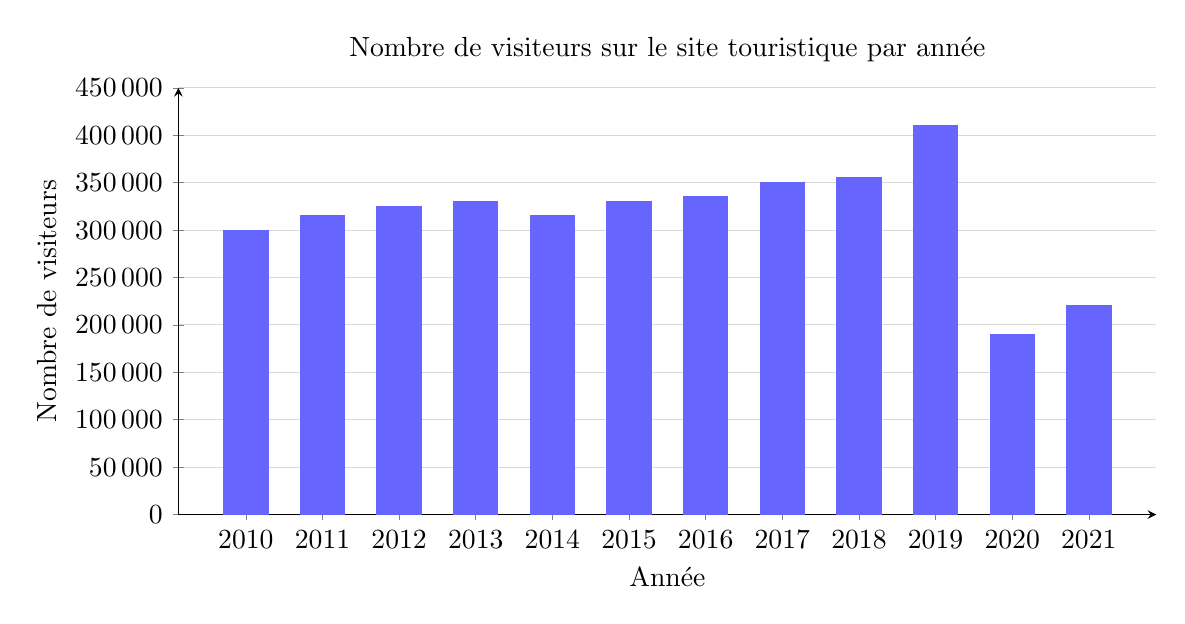
\begin{tikzpicture}
            \begin{axis}[
                ybar,
                axis lines=left,
                enlarge x limits=0.08,
                bar width=16pt,
                width=14cm,
                height=7cm,
                ymin=0, ymax=450000,
                ylabel={Nombre de visiteurs},
                xlabel={Année},
                symbolic x coords={2010,2011,2012,2013,2014,2015,2016,2017,2018,2019,2020,2021},
                xtick=data,
                title={Nombre de visiteurs sur le site touristique par année},
                ymajorgrids=true,
                grid style={gray!30},
                ytick distance=50000,
                scaled y ticks=false,
                yticklabel style={
                    /pgf/number format/fixed,
                    /pgf/number format/precision=0,
                    /pgf/number format/1000 sep={\,}
                }
            ]
            \addplot[
                fill=blue!60,
                draw=blue!60
            ] coordinates {
                (2010,300000)
                (2011,315000)
                (2012,325000)
                (2013,330000)
                (2014,315000)
                (2015,330000)
                (2016,335000)
                (2017,350000)
                (2018,355000)
                (2019,410000)
                (2020,190000)
                (2021,220000)
            };
            \end{axis}
        \end{tikzpicture}
    \end{center}
    \begin{enumerate}
        \item Quel a été le nombre de visiteurs en 2010~? \textit{Aucune
        justification n'est attendue.}
        \item En quelle année le nombre de visiteurs a-t-il été le plus élevé~?
        \textit{Aucune justification n'est attendue.}
    \end{enumerate}
    \item Le tableau ci-dessous indique le nombre de visiteurs sur le site
    touristique de cette ville en 2020 et en 2021.
    \begin{center}
        \begin{tblr}{colspec={Q[l,m]Q[c,m]Q[c,m]}, hlines, vlines}
            Année & 202 & 2021 \\
            Nombre de visiteurs & 187 216 & 219 042
        \end{tblr}
    \end{center}
    Le maire de cette ville avait pour objectif que le nombre de visiteurs
    progresse d'au moins 15 \% entre 2020 et 2021.\par\medskip\noindent
    L'objectif a-t-il été atteint~?\par\bigskip\noindent
    \textbf{Partie B : Étude des prix des hotels de cette ville.}\par\noindent
    Sur une période donnée, on relève les prix facturés pour une nuit par les
    hotles de cette ville.
    \begin{center}
        \begin{tblr}{colspec={Q[c,m,wd=60pt]*{8}{Q[c,m,wd=30pt]}}, hlines, vlines}
            Prix facturés pour une nuit (en euro)&60&80&85&90&110&120&350&500\\
            Effectif&1 200&1 350&1 000&1 100&1 200& 1300&900&300
        \end{tblr}
    \end{center}
    \item Déterminer l'étendue des prix facturés.
    \item Quelle est la moyenne des prix facturés pour une nuit~? Arrondir à
    l'euro près.
    \item L'association des hôteliers de cette ville cherche à attirer des
    touristes et annonce : \guillemets{Dans les hôtels de notre ville, au
    moins la moitié des nuits est facturé à moins de 100 \euro}. Est-ce vrai~?
\end{enumerate}
\showthesource
\end{document}